\section{Конструкторская часть}

В данном разделе описан разработанного метод и архитектуры системы, представлены механизмы защиты и примеры их использования для виртуализации функций доверенной среды исполнения.

\subsection{Описание архитектуры системы}

Разработанный метод предполагает использование принципа разделения функциональности на разные компоненты системы. Система спроектирована таким образом, что при атаке или получении доступа к одному из компонентов, её целостность нарушена не будет. Для корректной работы метода, система обязательно должна поддерживать технологию ARM TrustZone и аппаратные механизмы виртуализации ARM. 

Каждой гостевой виртуальной машине сопоставляется виртуальная машина выполняющая роль доверенной среды исполнения, для достижения данной цели используется гипервизор. Каждая виртуальная машина выполняется в обычном мире.

Для обеспечения целостности и проверки последовательности загрузки используется безопасный мир (с помощью ARM TrustZone). В безопасном мире располагаются модули управления таблицами трансляции гипервизора и виртуальных машин; модуль перехода и сохранения контекста между виртуальными машинами. Такой подход обеспечивает целостность данных, даже если код гипервизора был скомпрометирован.

Каждая ДСИ использует своё индивидуальное рабочее окружение, в котором хранятся данные. Окружение закреплено за конкретной виртуальной машиной и доступное только когда процессор выполняется в режиме hypervisor, с помощью чего и добивается изоляция. При этом, само окружение не является частью сущности гипервизора.

Для корректного и безопасного взаимодействия вышеописанных компонентов: модулей расположенных в безопасном мире, рабочих окружений и виртуальных машин используется отдельный модуль, который является частью гипервизора.

На рисунке \ref{fig:full-design} представлена схема разработанной системы.

\begin{figure}[h]
	\centering
	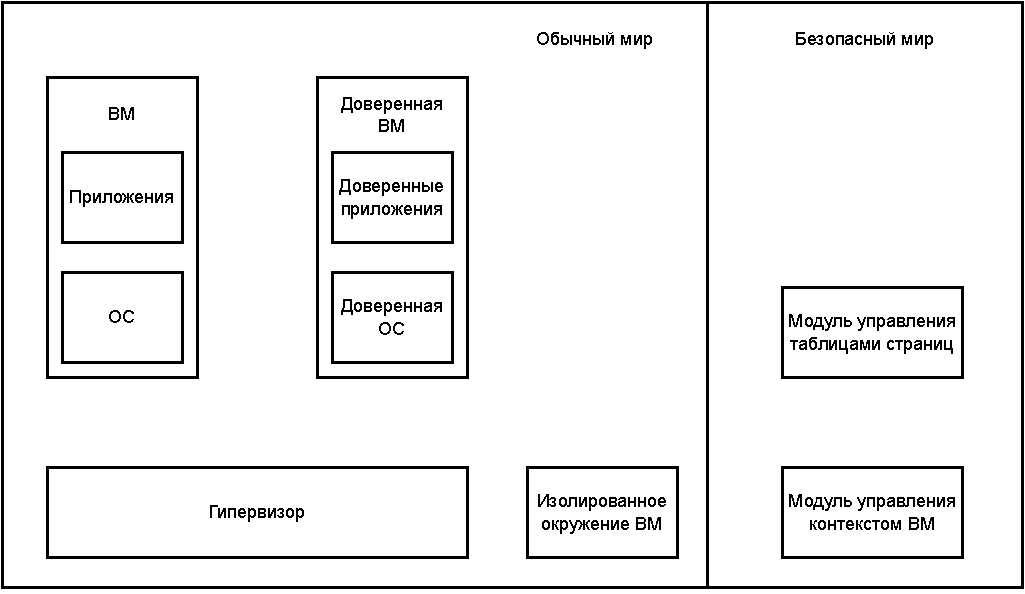
\includegraphics[width=\textwidth]{img/full-design.pdf}
	\caption{Концептуальная схема разработанной системы.}
	\label{fig:full-design}
\end{figure}

\subsection{Механизмы защиты}

\subsubsection{1}

\subsubsection{2}

\subsubsection{3}

\subsubsection{4}

\subsection{Виртуализация функций ДСИ}

\subsubsection{Доверенная загрузка}

\subsubsection{Состояние ядер процессора}

\subsubsection{Разделение ресурсов системы}

\pagebreak
